\subsubsection{E-Mail Spam Classification Using Long Short-Term Memory Method}
The research aimed to create a text-based dataset module architecture based on Multi Modal Architecture Model Fusion(MMA-MF) with the aim to be able to effectively filter spam even if it's hidden in text (\cite{dongre_patidar_2019}). The research argued that spammers had learned to evade the single model spam filtering systems by injecting junk information into the multi-modal part of an email thereby making the spam evade detection. This type of spam is called hybrid spam and they explained that it is more harmful than traditional spam since it contains more information than the latter thereby requiring more network bandwidth and storage space. The MMA-MF architecture combined both CNN and Long Short Term Memory (LSTM) to handle image and text data respectively to generate the class probabilities of the words and images in the email. A fully connected neural network with a logistic regressor at the output layer was added to the architecture to classify the class probabilities to either spam or ham (\cite{dongre_patidar_2019}).
Below is a figure of the architecture.
\begin{figure}[H]
    \centering
    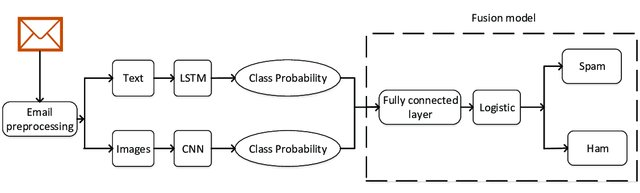
\includegraphics[width=13cm]{img/mma-mf.jpg}
    \caption{MMA-MF Architecture (\cite{dongre_patidar_2019})}
    \label{fig:hybrid_arch}
\end{figure}

The model was evaluated using 5-fold cross validation. Below is the performance of the model.

\begin{table}[H]
    \centering
    \begin{tabular}{|p{2cm}|p{2cm}|p{2cm}|p{2cm}|p{2cm}|}
         \hline
         Fold & Accuracy & Recall & F1-Score & Precision  \\
         \hline
         \multicolumn{5}{|c|}{MMA-MF Model for Text Dataset 1}\\
         \hline
         1 & 98.42 & 97.64 & 97.24 & 98.5 \\
         \hline
         2 & 98.67 & 98.15 & 97.47 & 98.5 \\
         \hline
         3 & 98.67 & 98.19 & 97.65 & 99 \\
         \hline
         4 & 98.25 & 97.71 & 97.27 & 98 \\
         \hline
         5 & 98.42 & 97.89 & 97.53 & 98.5 \\
         \hline
         \multicolumn{5}{|c|}{MMA-MF Model for Text Dataset 2}\\
         \hline
         1 & 93.35 & 92.64 & 92.89 & 90.5 \\
         \hline
         2 & 92.56 & 92.63 & 92.75 & 90.01 \\
         \hline
         3 & 91.5 & 92.33 & 91.83 & 93.5 \\
         \hline
         4 & 92.35 & 92.83 & 92.97 & 92 \\
         \hline
         5 & 93.44 & 92.72 & 92.71 & 92.5 \\
         \hline
    \end{tabular}
    \caption{Fold Cross-Validation Chart for Text Dataset 1 and 2}
    \label{tab:mma-mf}
\end{table}